\documentclass{article}
\usepackage[utf8]{inputenc}
\usepackage{amsmath}
\usepackage{amsfonts}
\usepackage{amssymb}
\usepackage{graphicx}
\usepackage{algorithm}
\usepackage{algpseudocode}
\usepackage{blindtext}
\usepackage{hyperref}
\usepackage{amsthm}

\newtheorem{theorem}{Theorem}

\title{Statistical independence measure based on maximum norm of joint and product-marginal characteristic functions}
\author{povilas.daniusis, povilasd@neurotechnology.com}
\date{November 2021}

\begin{document}
\maketitle

% 1. Artificial data experiments: additive, multiplicative noise, noise effect, scale invariance.
% 2. Classification experiments.
%

\begin{abstract}
    In this paper we propose statistical independence measure based on the maximum norm of difference between joint and product of marginal characteristic functions. We discuss simulated examples, and applications for feature selection/extraction, causal inference and conduct corresponding empirical experiments with diverse collection of data sets from different domains.
\end{abstract}

\section{Introduction}
Statistical dependence measures plays important role in various statistical and machine learning methods (e.g. hypothesis testing~\cite{Gretton2005MeasuringSD}, feature selection and extraction~\cite{EigenHSIC}, information bottleneck methods \cite{Ma2020TheHB}, causal inference~\cite{NIPS2008_f7664060}, self-supervised learning~\cite{li2021selfsupervised}, causal inference~\cite{NIPS2008_f7664060}, among others).  Earliest statistical dependence estimation ideas (e.g. conditional probability) share nearly-common origin with the beginning of formal statistical reasoning itself. During last two centuries ideas of correlation and (relative) entropy (including various generalizations) were proposed and became very popular in numerous applications and theoretical developments. However, with the increasing popularity of statistical machine learning, new statistical dependence estimation methods, that are robust, applicable to noisy, high-dimensional, structured data, and which can be efficiently integrated with modern machine learning methods are helpful for the development both of the theory and application.

In this article we focus on quantitative estimation of statistical independence, using characteristic functions. We begin with the short review of some important previous dependence estimation approaches (Section~\ref{section:previous_work}), devoting special attention to ones based on characteristic functions (Section~\ref{section:previous_work_cf}). Afterwards we formulate new characteristic function-based statistical dependence measure and its empirical estimator (Section~\ref{section:proposed_method}), including its extension into reproducing kernel Hilbert spaces (RKHS'es), which are the main theoretical contribution of our paper. Section~\ref{section:experiments} is devoted to experiments with simulated and real data sets, and finalizing Section~\ref{section:discussion} concludes this article.

\section{Previous work}
\label{section:previous_work}
Shannon mutual information~\cite{Cover2006} and generalizations ~\cite{e20110813},  Hilbert-Schmidt independence criterion \cite{Gretton2005MeasuringSD} and generalizatios~\cite{?}, \cite{Pczos2012CopulabasedKD} copula-based kernel dependence measures.

\subsection{Characteristic-function-based methods}
\label{section:previous_work_cf}
Characteristic function of $d_{X}$-dimensional random vector $X$ defined in some probability space $(\Omega_{X}, \Sigma_{X}, \mathbb{P}_{X})$ is defined as 
\begin{equation}
    \label{eq:characteristic_function}
    \phi_{X}(\alpha) = \mathbb{E}_{X} e^{i\alpha^{T}X}, 
\end{equation}
where $i=\sqrt{-1}$, $\alpha \in R^{d_{X}}$. Having $n$ i.i.d. realisations of $X$, corresponding empirical characteristic function is defined as
\begin{equation}
    \label{eq:ecf}
  \widehat{\phi_{X}}(\alpha) = \frac{1}{n} \sum_{j=1}^{n} e^{i <\alpha, x_{j}>}.
\end{equation}
Having pair of two random vectors $(X,Y)$ defined in another probability space $(\Omega_{X,Y}, \Sigma_{X,Y}, \mathbb{P}_{X,Y})$  joint characteristic function is defined as:
\begin{equation}
    \label{eq:joint_characteristic_function}
    \phi_{X,Y}(\alpha,\beta) = \mathbb{E}_{X,Y} e^{i(\alpha^{T}X + \beta^{T}Y)},
\end{equation}
where $\alpha \in R^{d_{X}}$ and $\beta \in R^{d_{Y}}$. Similarly, having 
$n$ i.i.d. realisations of $(X,Y)$, joint empirical characteristic function is defined as
\begin{equation}
    \label{eq:joint_ecf}
\widehat{\phi_{X,Y}}(\alpha,\beta) = \frac{1}{n} \sum_{j=1}^{n} e^{i(<\alpha, x_{j}> + <\beta, y_{j}>) }.
\end{equation}

In terms of characteristic functions, statistical independence  of $X$ and $Y$ is equivalent to $\forall \alpha \in R^{d_x},\forall \beta \in R^{d_y} $, 

\begin{equation}
%\mathbb{E}_{X,Y} e^{i <\alpha, X> + i <\beta, Y>} = \mathbb{E}_{X} e^{i <\alpha, X>} \mathbb{E}_{Y} e^{i <\beta, Y>},
\label{eq:kac_theorem}
\Delta_{X,Y}(\alpha, \beta) := \phi_{X,Y}(\alpha,\beta) - \phi_{X}(\alpha) \phi_{Y}(\beta) = 0,
\end{equation}
where $d_{x}$ and $d_{y}$ are dimensions of $X$ and $Y$, respectively.

This formulation of statistical independence was used as the basis (first in~\cite{Feuerverger} for univariate case, and afterwards extended and developed by~\cite{Szekely} for bivariate multidimensional random vectors) for construction of statistical independence tests and measures.\textit{Distance covariance} and \textit{distance correlation}, prosposed by ~\cite{Szekely} relies on weighted $L^{2}$-norm analysis of~\eqref{eq:kac_theorem}. They select weighting function in such a way, that dependence measure can be expressed in terms of correlection of data-dependent distances. Study~\cite{Bottcher} generalises~\cite{Szekely} to multivariable case and proposes \textit{distance multivariance} and derivative dependence measure, called~\textit{total distance multivariance}. 

Our motivation stems from the fact that evaluation of~\cite{Szekely} measures in high dimensional cases may be prone to curse of dimensionality (as mentioned in~\cite{Edlemann}). Although staying in $L^{p}$-space framework, insted of $p = 2$ ($L^{2}$ space) we take a limit when  $p \rightarrow \infty$, and also avoid direct calculation of integral by working in $L^{\infty}$, which has corresponding supremum norm. Also, from practical point of view maximization is convenient, because it is already implemented in various deep learning frameworks. %\textit{What are potential advantages of maximum norm?}

\section{Proposed Independence Measure}
\label{section:proposed_method}
% sparse vectors - PAC style theorem ?



\noindent This motivates the construction of a novel dependence measure, which we further refer to as Kac independence measure (KacIM). Let $X$ and $Y$ be two standartized random random vectors. The proposed independence measure is defined as
\begin{equation}
\label{eq:kim}
    \kappa(X,Y) = \max_{\alpha \in \mathbb{R}^{d_{X}}, \beta \in \mathbb{R}^{d_{Y}}} \vert \phi_{X,Y}(\alpha, \beta)  -\phi_{X}(\alpha) \phi_{Y}(\beta) \vert.
\end{equation}

%In contrary to~\cite{Szekely} the proposed~\eqref{eq:kim} measure relies on maximum norm of difference between joint and product-marginal characteristic functions.

\subsection{Properties}
\begin{theorem}
\label{thm:properties}
  Statistical independence measure~\eqref{eq:kim} has the following properties:
  \begin{itemize} 
    \item $\kappa(X,Y) = \kappa(Y,X)$,
    \item $0 \leq \kappa(X,Y) \leq 1$,
    \item $\kappa(X,Y) = 0$ iff $X\perp Y$.
   \end{itemize}    
\end{theorem}


\begin{proof}
\textit{Proof}
Symmetry is obvious from definition~\eqref{eq:kim} (commutativity of addition and multiplication), and second property directly follows from Cauchy inequality and that absolute value of characteristic function is bounded by $1$:
\begin{multline*}
|\phi_{X,Y}(\alpha, \beta)  -\phi_{X}(\alpha) \phi_{Y}(\beta)|^{2} =
\mathbb{E}_{X,Y} |( e^{i\alpha^{T}X} - \phi_{X}(\alpha) )(e^{i\beta^{T}Y}- \phi_{Y}(\beta) )|^{2} = \\
\mathbb{E}_{X,Y} |( e^{i\alpha^{T}X} - \phi_{X}(\alpha) )|^{2} |(e^{i\beta^{T}Y}- \phi_{Y}(\beta) )|^{2}  = (1 - |\phi_{X}(\alpha)|^{2}) (1 - |\phi_{Y}(\beta)|^{2}).
\end{multline*}
\end{proof}

%\paragraph{Scale invariance}
%$\kappa(\lambda X, \lambda Y) = \max_{\|\alpha\| = \|\beta\| = 1} \vert \phi_{\lambda X,\lambda Y}(\alpha + \beta)  -\phi_{\lambda X}(\alpha) \phi_{\lambda Y}(\beta)\vert = \max_{\\|\lambda \alpha\| = \|\lambda \beta\| = 1} \vert \phi_{X,Y}(\lambda(\alpha + \beta))  -\phi_{X}(\lambda\alpha) \phi_{Y}(\lambda\beta) \vert = \max_{\\|s\| = \|t\| = 1} \vert \phi_{X,Y}(s+t)  -\phi_{X}(s) \phi_{Y}(t) \vert = \kappa( X, Y). ?$

\subsection{Estimation}

Having i.i.d. standartized data $(x_{j}, y_{j})$, $j = 1,2,...,n$, an empirical scale-invariant estimator of~\eqref{eq:kim} is defined via corresponding empirical characteristic functions~\eqref{eq:joint_ecf} and~\eqref{eq:ecf}:
\begin{equation}
\label{eq:estimator}
    \hat{\kappa}(X,Y) = \max_{\|\alpha\| = \|\beta\| = 1} \vert \widehat{\phi_{X,Y}}(\alpha,\beta)  - \widehat{\phi_{X}}(\alpha) \widehat{\phi_{Y}}(\beta) \vert.
\end{equation}

\noindent Empirical estimator~\eqref{eq:estimator} also is symmetric and and bounded (Theorem~\ref{thm:properties}) . Normalisation of parameters $\alpha$ and $\beta$ on to unit sphere is included due to stability issues (really this is the reason?). The  estimator~\eqref{eq:estimator} can be calculated by using Algorithm~\ref{alg:estimator_computation} \footnote{ Pytorch~\cite{NEURIPS2019_9015} implementationcan be accessed from \url{https://github.com/povidanius/kac_independence_measure}}. 

\begin{algorithm}
\caption{KacIM estimator computation algorithm}\label{alg:estimator_computation}
\begin{algorithmic}
\Require data batch $(x,y)$, gradient-based optimiser $GradOpt(loss)$
%\Ensure $y = x^n$
\State Normalize $(x,y)$ to zero mean and unit variance (scale invariance).
\State Calculate KacIM estimator $\hat{\kappa}(x,y)$, without maximization step (i.e. using current $\alpha, \beta$).
\State Perform one maximization iteration of computed $\hat{\kappa}(x,y)$ via $\alpha, \beta \rightarrow GradOpt(\hat{\kappa}(x,y))$.
\end{algorithmic}
\end{algorithm}
In our implementation we use decoupled weight decay regularization optimizer~\cite{Loshchilov2019DecoupledWD}.

\subsection{Kernel version}

Having two RKHS'es, defined by feature mapping $(x,y) \rightarrow (\l(x,.), \l(y,.)$, where $k: \mathbb{R}^{d_{x}} \times \mathbb{R}^{d_{x}} \rightarrow \mathbb{R}$ and $l: \mathbb{R}^{d_{y}} \times \mathbb{R}^{d_{y}} \rightarrow \mathbb{R}$ (see~\cite{10.5555/3279302}). Then, estimation of kernel-$KIM$ ($\hat{\kappa}_{k,l} (X,Y)$) can be reformulated as maximization of :
\begin{equation}
\label{eq:kernel_estimator}
    \vert \frac{1}{n} \sum_{j=1}^{n} e^{i(<\alpha, k(x_{j},.)> + <\beta, l(y_{j}>,.)) } - \frac{1}{n^2} \sum_{j=1}^{n} e^{i <\alpha, k(x_{j},.)>}\sum_{k=1}^{n} e^{i<\beta, l(y_{k},.)>}\vert,
\end{equation}

and representer theorem\cite{?} implies 

\begin{equation}
\label{eq:kernel_estimator1}
    \hat{\kappa}_{k,l} (X,Y) = \max_{\|\alpha\| = \|\beta\| = 1} \vert \frac{1}{n} 1^{T} e^{i(\alpha^{T} K + \beta^{T} L)} - \frac{1}{n^2} (1^{T} e^{i(\alpha^{T}K)}) (1^{T} e^{i(\beta^{T}L)}) \vert,
\end{equation}

where $K$ and $L$ are Gram matrices, corresponding to $x_{i}$ and $y_{i}$. Note that the number of parameters of $\hat{\kappa}_{k,l} (X,Y)$ is dimension-idnependent and is equal to $2n_{b}$, where $n_{b}$ is batch size. Also, kernel-$KIM$ can be applied for structured data, via corresponding positive defined kernels.

\section{Experiments}
\label{section:experiments}
Dependence measures have board area of applications (e.g.~\cite{WANG2021107567}). For example, regularization~\cite{?,?}, feature selection and extraction~\cite{EigenHSIC}, information bottleneck methods \cite{Ma2020TheHB}, causal inference~\cite{NIPS2008_f7664060}, among others. Further we will conduct empirical investigation of KacIM. Starting with simple illustrative simulations, we will reformulate some key ideas in aforementioned topics for KacIM, and experimentally investigate corresponding empirical scenarios.


\subsection{Generated data}

We begin with simple example, which demonstrates the efficiency of KacIM for simulated multivariate data with additive and multiplicative noise.

\begin{figure}[t]
\label{fig:experiments_simulation}
\centering
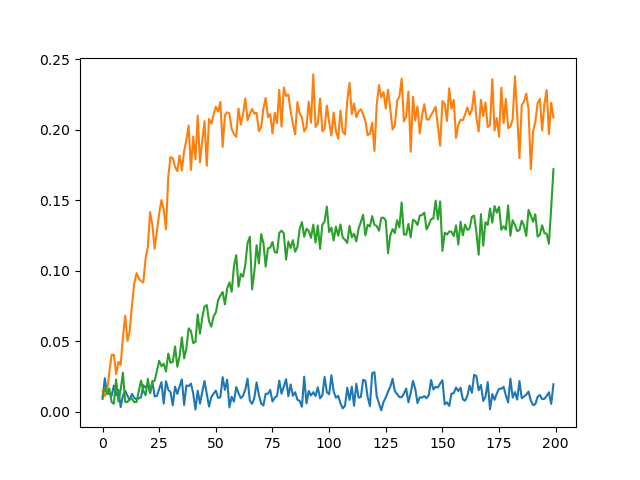
\includegraphics[scale=0.35]{../experiments/basic_demonstration/dependence_detection.png}
\caption{Dependence detection in independent data (blue), additive (orange) and multiplicative (green) noise scenarios.}
\end{figure}

In Figure~\ref{fig:experiments_simulation} reflects KacIM values during iterative adaptation ($200$ iterations). In the case of independent data, both $x_{i}$ and $y_{i}$ ($d_{x} = 512$, $d_{y} = 4$) are sampled from gaussian distribution, independently. In the case of dependent data, an additive noise (left graph) and multiplicative noise (right graph), the dependent variable is generated according to $y_{i} = sin(P x_{i}) + cos(P x_{i}) + \lambda \epsilon_{i}$ ($\lambda = 1.00$) and $y_{i} = (sin(P x_{i}) + cos(P x_{i})) \epsilon_{i}$, respectively, where $P$ is $d_{x} \times d_{y}$ random projection matrix, $\epsilon_{i} \sim N(0,1)$ and $\epsilon_{i} \perp x_{i}$.

When data is independent (blue graph), both in additive and multiplicative cases, due to independence, estimator~\eqref{eq:estimator} is resistant to maximization, and oscillates near zero. On the other hand, when data is not independent (orange and green graphs), the condition~\eqref{eq:kac_theorem} is violated and maximization of estimator~\eqref{eq:estimator} is possible.
%\subsection{Influence of noise variance and data scale}
\paragraph{Noise variance} In this simulation we use the same additive noise setting as in previous paragraph, but evaluate all noise levels $\lambda \in [0.1, 3.0]$, with step $0.1$.
Figure~\ref{fig:experiments_noise_level_effect} empirically shows that value of KacIM  negatively correlates with noise level, and therefore the proposed measure is able not only to detect whether independence is present, but also to quantitatively evaluate it, which enables to use it to derive cost functions for various learning-based algorithms. 

Since in~\ref{alg:estimator_computation} we standartize data, KacIM is also scale-invariant (i.e. $\kappa(rx, ry) = \kappa(x,y)$), where $r>0$ is scale parameter.

\begin{figure}[t]
	\label{fig:experiments_noise_level_effect}
	\centering
	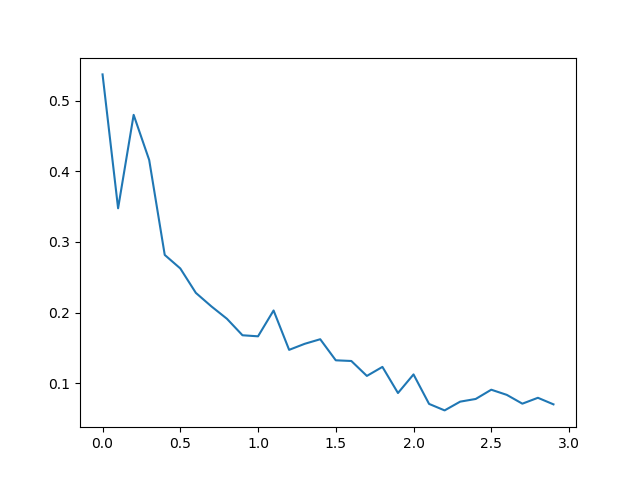
\includegraphics[scale=0.30]{./summary_noise_effect.png}
	\caption{Noise level ($x$ axis) vs final iteration KacIM value ($y$ axis). KacIM values for larger noise levels saturates as in tail of graph.}
\end{figure}



\subsection{Feature Extraction}

We conduct linear feature extraction by seeking 

\begin{equation}
\label{eq:kim_feature_extraction}    
W^{*} = arg \max_{W} \kappa(Wx, y) - \alpha Tr\{(W^{T}W-I)^{T}(W^{T}W-I) \},
\end{equation}
where the regularisation term, controlled by multiplier $\alpha \geq 0$, enforces projection matrix $W^{*}$ to be orthogonal.

%\begin{equation}
%\label{eq:kim_feature_extraction1}    
%w_{t}^{*} = arg \max_{W} \frac{\kappa(w_{t}^{T}x, y)}{\kappa(w_{t}^{T}x, W_{t}x)}.
%\end{equation}

\noindent Afterwards, feature extraction is conducted by $f = W^{*}x$ and these features are used as the inputs to several popular classifiers ($k$-nearest neighbor classifier with Euclidean distance, logistic regression, linear and quadratic support vector machine\cite{?}). We randomly split all the datasets in training and testing sets of equal size, comparing unmodified inputs $x$, and features of all possible dimensions up to $d_{x}$.  In our experiments we set $\alpha$ to $1.0$ to quickly ensure orthogonal projection matrices, and further proceed to dependence maximization stage. 
The classification accuracies, reported in~\ref{table:classification_accuracies} demonstrate that this KacIM-based feature extraction procedure indeed allows to increase classification accuracy when applied to real data sets from various domains.

\begin{table}
\label{table:classification_accuracies}	
\begin{tabular}{ |p{2.5cm}||p{2cm}|p{1cm}|p{1cm}|p{1cm}|  }
	\hline
	\multicolumn{5}{|c|}{Classification accuracies} \\
	\hline
	Dataset & KNN(3) & LR & LSVM & QSVM  \\
	\hline
	Ionosphere   & AF    &AFG&   004 & \\	
	\hline
	Spambase & & & & \\
	\hline
	One-hundred-plants-texture   & AF    &AFG&   004 & \\
	\hline
\end{tabular}
\end{table}
\section{Discussion} 

\label{section:discussion}
In this article we propose statistical dependence measure, KacIM, which relies on simple fact that statistical independence is equivalent to the decomposability of joint characteristic function  into the product of marginal ones. Although we formulated and analysed KacIM for bivariate vectorial case, similarly it can be generalised for multivariate case. In addition, since characteristic functions are defined for matrices, graphs, and other objects \cite{?}, likely KacIM can be extended to those objects as well, which is potential direction of future research of KacIM.

Empirical analysis show, that KacIM can detect and measure statistical independence for non-linearly related, high-dimensional data. (...)

\section{Acknowledgements}


%\subsection{KacIM for information bottleneck}
%\subsection{Canonical component analysis, independent component analysis}
%\subsection{Causal inference}
%\subsection{Electroencephalography (?)}
%\section{Notes}
%Compare with  mutual information.


%\bibliographystyle{apalike}
\bibliographystyle{unsrt}

{\footnotesize
\bibliography{bibliography}}

% https://arxiv.org/pdf/2104.06612.pdf

%\begin{thebibliography}{}
%\bibitem{KacTheorem} David Applebaum, B.V. Rajarama Bhat, Johan Kustermans, J. Martin Lindsay, Michael Schuermann, Uwe Franz: Quantum Independent Increment Processes I: From Classical Probability to Quantum Stochastic Calculus
%\end{thebibliography}

\end{document}
